\documentclass{beamer}

\usepackage[utf8]{inputenc}
\usepackage[english]{babel}
\usepackage{tikz}
\usepackage{mathtools}
\usepackage{multirow}
\usepackage{anyfontsize}
\usepackage{amsmath}
\usepackage{amssymb}
\usepackage{algorithm}
\usepackage{algpseudocode}
\usepackage{bm}
\graphicspath{{imgs/}}

\usepackage{pgf,tikz}
\usepackage{localpie}

\newcommand{\NN}{\ensuremath{\mathbb N}}
\newcommand{\ZZ}{\ensuremath{\mathbb Z}}
\newcommand{\QQ}{\ensuremath{\mathbb Q}}
\newcommand{\RR}{\ensuremath{\mathbb R}}
\newcommand{\CC}{\ensuremath{\mathbb C}}
\newcommand{\LL}{\ensuremath{\mathbb L}}
\newcommand{\PP}{\ensuremath{\mathbb P}}

\usetheme{Ilmenau}
\usecolortheme{beaver}

\setbeamerfont{itemize/enumerate subbody}{size=\scriptsize}

\newcommand{\unit}[1]{\ensuremath{\:\text{#1}}}
\newcommand{\pro}{\ensuremath{\unit{\%{}}}}

\expandafter\def\expandafter\insertshorttitle\expandafter{%
  \insertshorttitle\hfill%
  \insertframenumber\,/\,\inserttotalframenumber}

\setbeamertemplate{itemize item}[square]
\setbeamertemplate{itemize subitem}[circle]
\setbeamertemplate{enumerate item}[square]

\title{20 Raspberry Pi's, One Model}

\subtitle{
    Federated Learning On Real Hardware
}
\author[Søren Holm, Asger Schultz, Gustav Moesmand]
{Søren Winkel Holm, Asger Laurits Schultz, Gustav Lang Moesmand}
\institute[DTU]{Technical University of Denmark}
\date{\today}

\begin{document}
\begin{frame}
    \titlepage
\end{frame}

\begin{frame}
    \frametitle{The Presentation}
    \footnotesize
    \tableofcontents
\end{frame}

\section{The Federated Learning Problem}
\begin{frame}
	\frametitle{Introduction}
	\noindent
	\begin{columns}
		\begin{column}{.5\textwidth}
			\begin{itemize}
				\item Multiple clients collaborate to generate global model
				%\item Pioneered by Google motivated by privacy and size of data sets
				\item Literature often benchmarks on central compute clusters
				\item How does physical devices impact performance?
			\end{itemize}
		\end{column}
		\begin{column}{.5\textwidth}
			\begin{figure}
    				\centering
				\scalebox{.6}{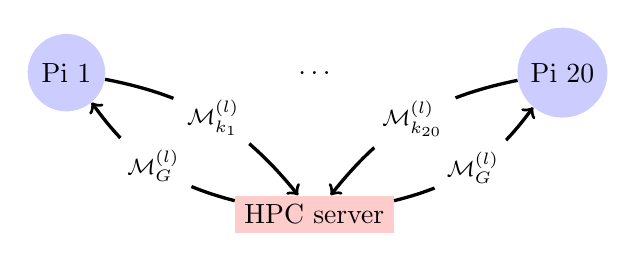
\begin{tikzpicture}[scale=.9,auto=center,every node/.style={circle}]

\tikzstyle{client}=[fill=blue!20];
\tikzstyle{server}=[fill=red!20,style=rectangle];
\tikzstyle{t}=[fill=red!0];

\node[server] (s) at (0,0) {HPC server};  
\node[client] (c1) at (-3.5,2)  {Pi $1$}; 
\node[t] (te) at (0, 2) {$\ldots$};
\node[client] (c2) at (3.5,2)  {Pi $20$};  

\path[->] (s) edge[very thick, bend left=20] node[midway, fill=white] {\footnotesize $\mathcal M_G^{(l)}$} (c1);
\path[->] (s) edge[very thick, bend right=20] node[midway, fill=white] {\footnotesize $\mathcal M_G^{(l)}$} (c2);

\path[->] (c1) edge[very thick, bend left=20] node[midway, fill=white] {\footnotesize $\mathcal M_{k_1}^{(l)}$} (s); 
\path[->] (c2) edge[very thick, bend right=20] node[midway, fill=white] {\footnotesize $\mathcal M_{k_{20}}^{(l)}$} (s); 


\end{tikzpicture}
}
			\end{figure}
		\end{column}
	\end{columns}
\end{frame}

\begin{frame}
	\frametitle{Motivation}
	% \begin{columns}
	% 	\begin{column}{.5\textwidth}
			\begin{itemize}
				\item Seek to capture problems and trade-offs when using physical hardware
				\item Study key hyperparameters of the FedAvg algorithm
				\item Implement and use a stronger aggregation scheme (FedDF) and compare it agains FedAvg
			\end{itemize}
		% \end{column}
	% \end{columns}
\end{frame}

\begin{frame}
    \frametitle{Real-Life Setup}
    \noindent
    \begin{columns}
	    \begin{column}{.5\textwidth}
		    \begin{itemize}
			    \item Setup consists of 20 Raspberry Pies 
			    \item Both Ethernet and Wifi capability to test for different amounts of network overhead
			    \item 40 clients, where up to 20 can be assigned to a Pi each communication round
				    \begin{itemize}
					    \item Each client is a unique subset of the dataset
				    \end{itemize}
		    \end{itemize}    
	    \end{column}
	    \begin{column}{.5\textwidth}
		    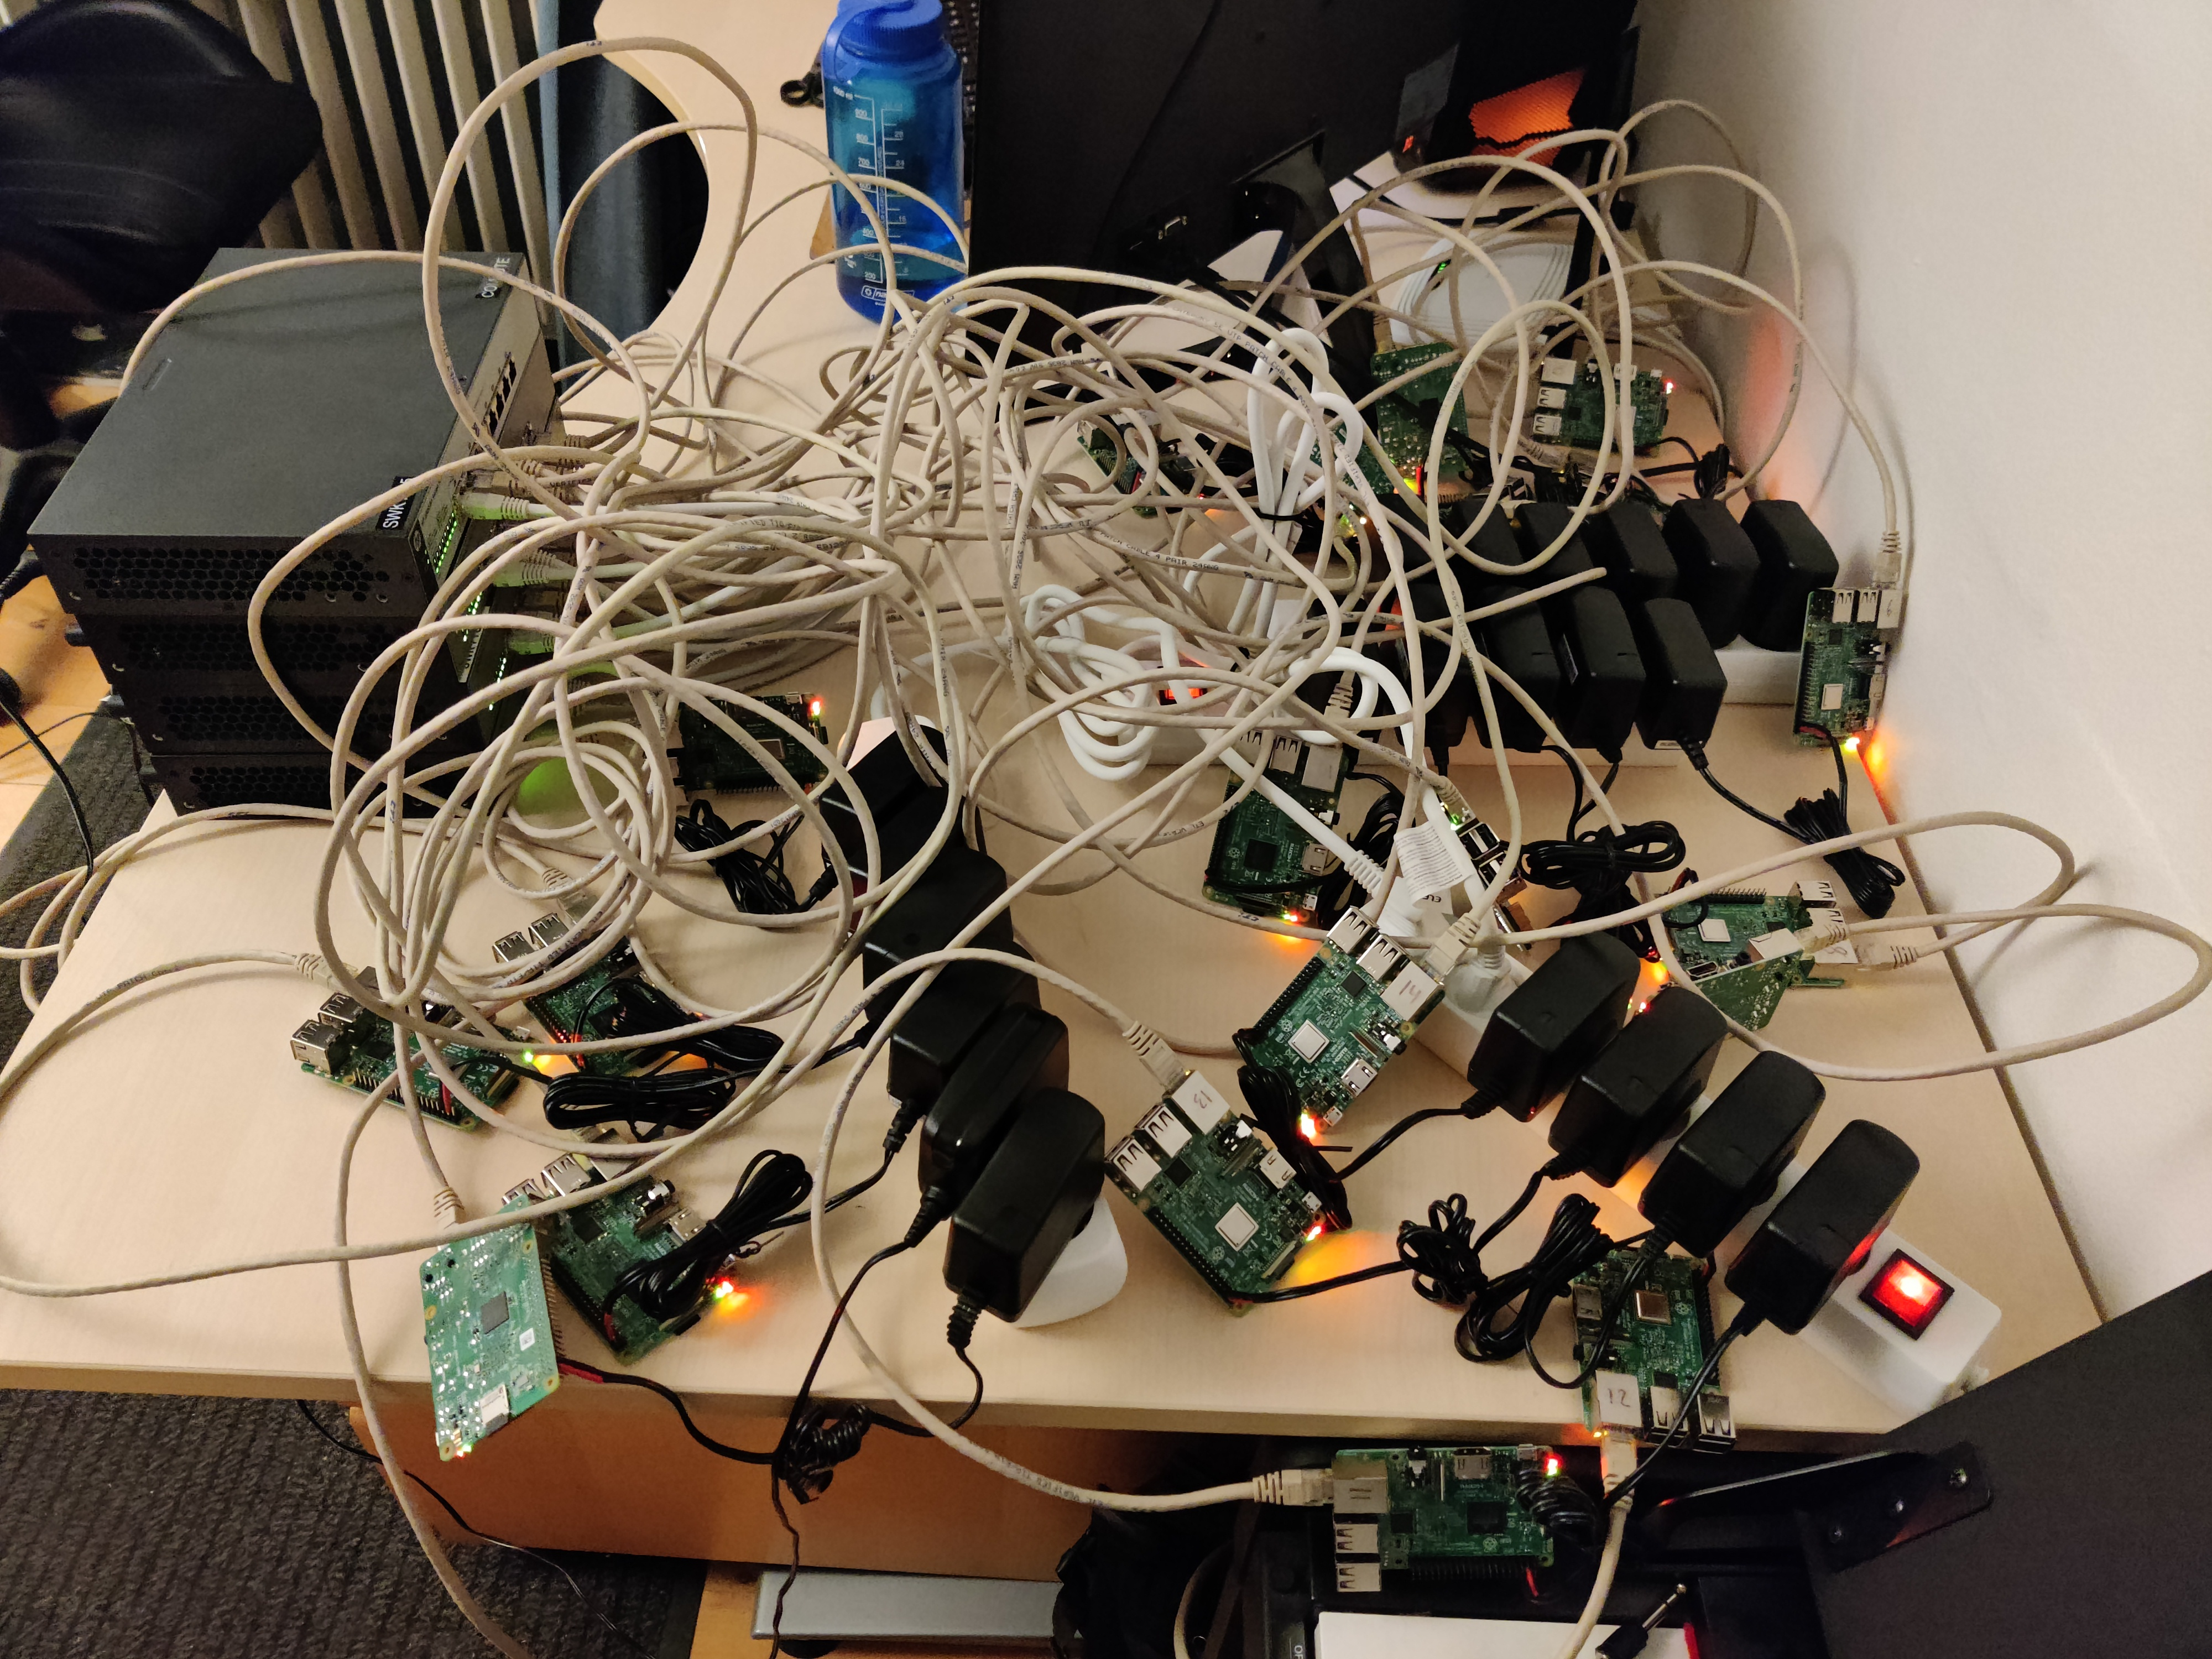
\includegraphics[width=1\textwidth]{imgs/IMG_20220322_214443}
	    \end{column}
    \end{columns}
\end{frame}

\begin{frame}
	\frametitle{The Learning Problem}	
	\noindent
	\begin{columns}
		\begin{column}{.5\textwidth}
			\begin{itemize}
				\item CIFAR-10 transformed to greyscale
				\item Model
					\begin{itemize}
						\item 2 convolutional layers
						\item 2 linear layers
					\end{itemize}
				\item Adam optimizer
                                \item Learning rate decay
			\end{itemize}
		\end{column}
		\begin{column}{.5\textwidth} 
			\begin{figure}
				\centering
				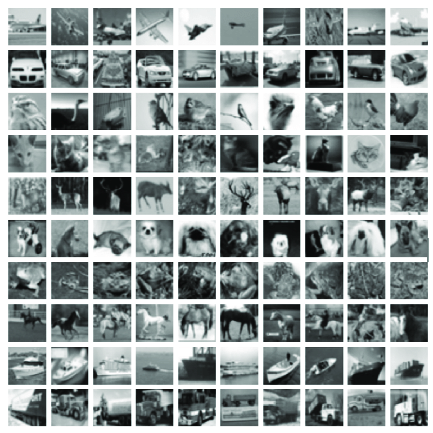
\includegraphics[width=\textwidth]{imgs/cifar10-greyscale.png}
			\end{figure}
		\end{column}	
	\end{columns}
\end{frame}

\begin{frame}
	\frametitle{Unbalanced data}
	\noindent
	\begin{columns}
		\begin{column}{.45\textwidth}
			\begin{itemize}
				\item Real world data spread across clients are bound to be unbalanced
				\item To simulate this we use Dirichlet sampling
				\item One key parameter $\alpha$
					\begin{itemize}
						\item $\alpha \to 0$ leads to imbalance
						\item $\alpha \to \infty$ leads to balance
						\item Default for all experiments: $\alpha=1$
					\end{itemize}
			\end{itemize}
		\end{column}
		\begin{column}{.55\textwidth}
			\begin{figure}[htb!]
				\centering
				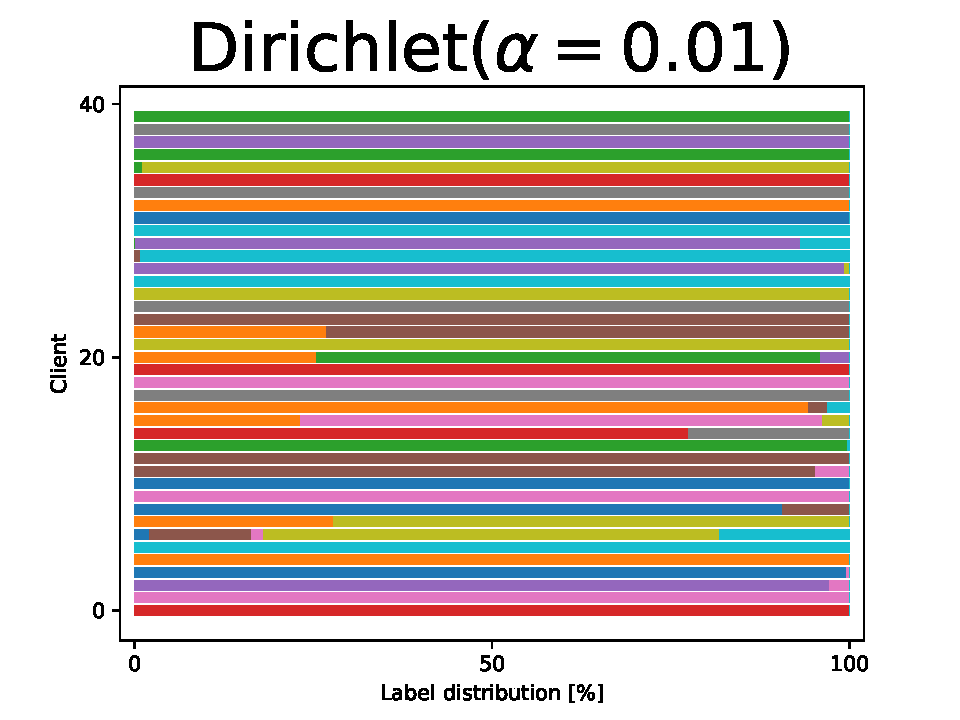
\includegraphics[width=0.49\linewidth]{imgs/splits(alpha=0.01)}
				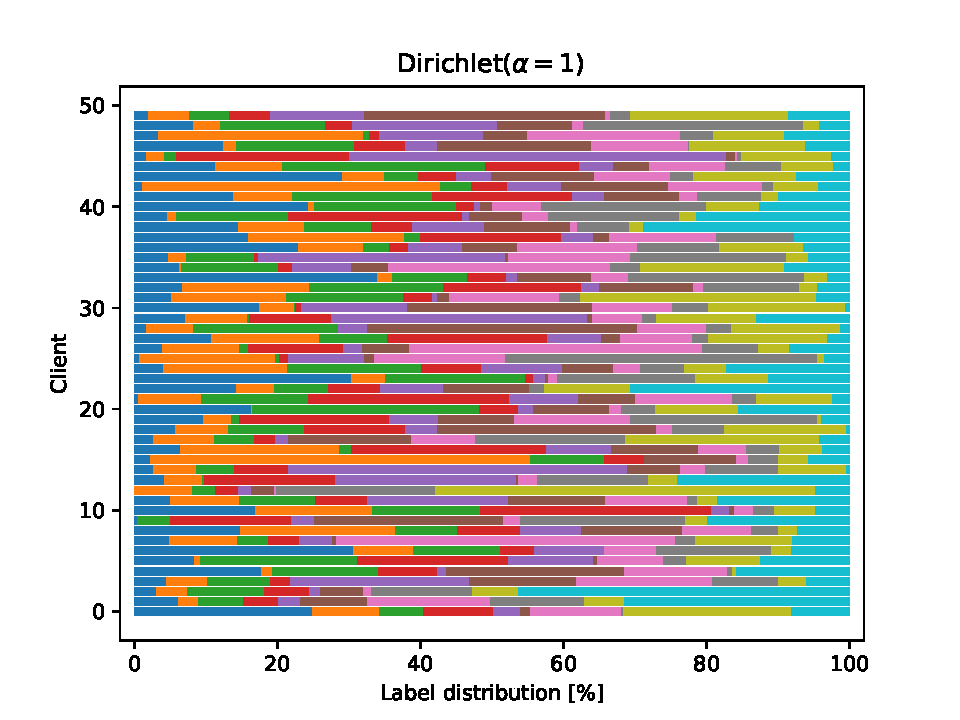
\includegraphics[width=0.49\linewidth]{imgs/splits(alpha=1).pdf}
				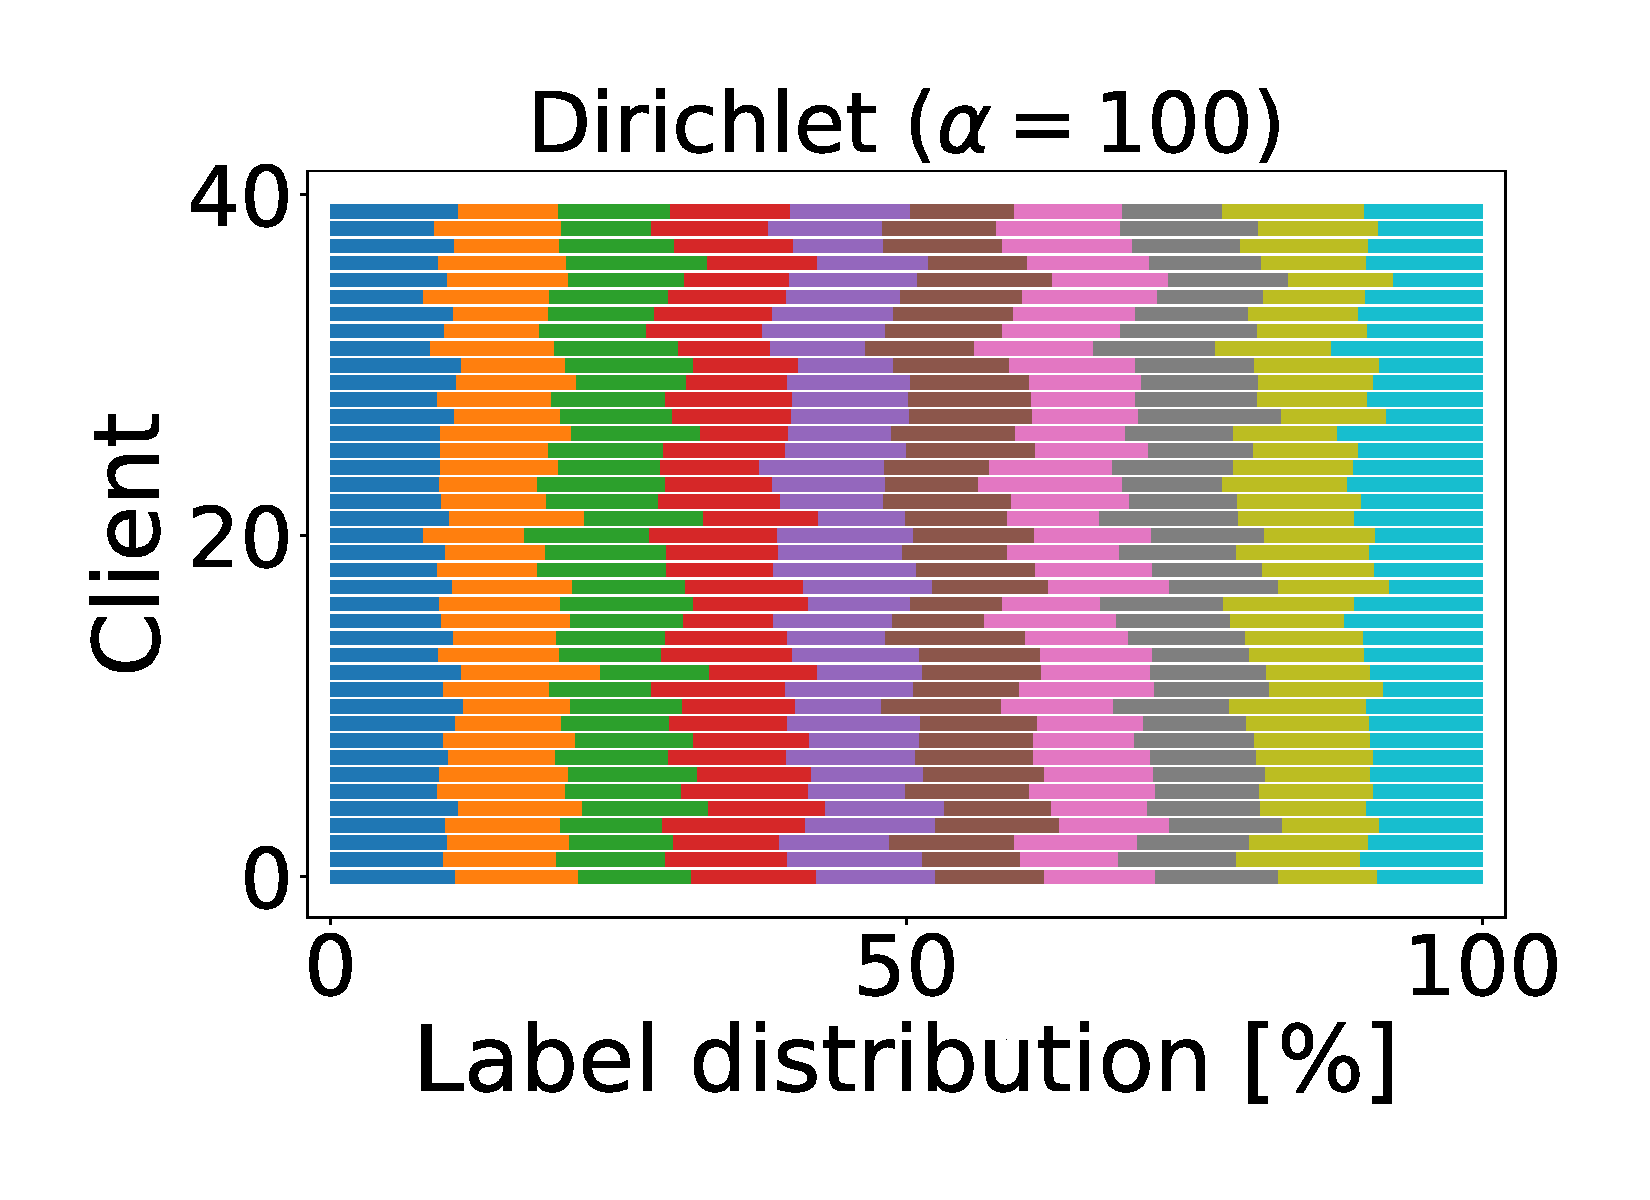
\includegraphics[width=0.49\linewidth]{imgs/splits(alpha=100)}
				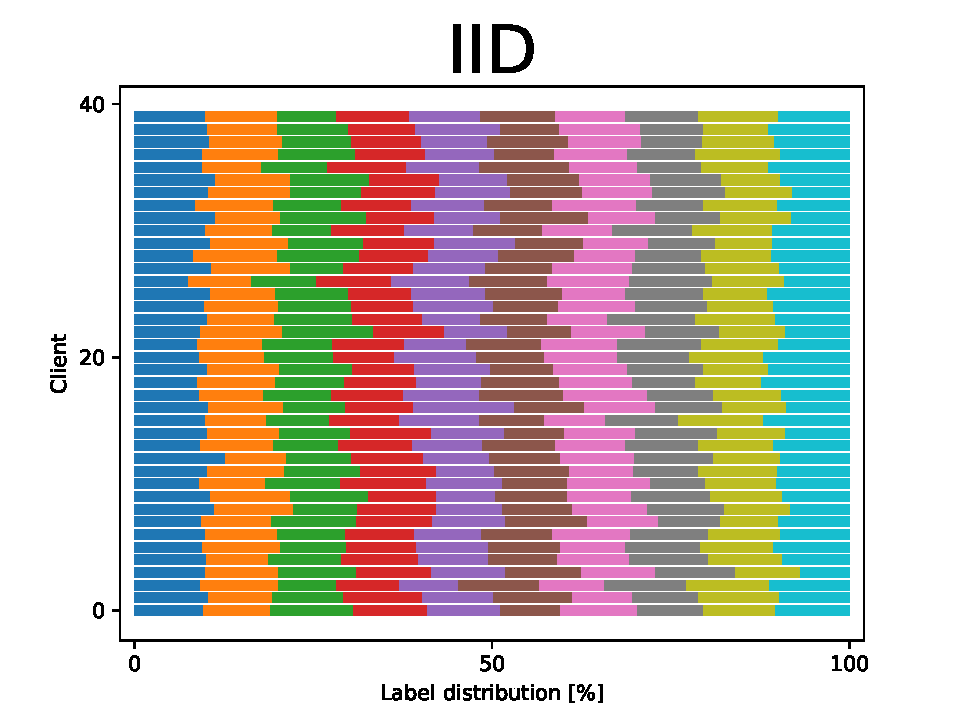
\includegraphics[width=0.49\linewidth]{imgs/splits(IID)}
			\end{figure}
		\end{column}
	\end{columns}

\end{frame}

\section{FedAvg on Real Hardware}
\begin{frame}
    \frametitle{FedAvg: The Simple Algorithm [2]}
    \begin{enumerate}
        \item Initialize global model, $\mathcal M_G$
        \item Distribute to $S \le K$ randomly sampled devices
        \item On each client $s$, train local model $\mathcal M_s$ for $E$ epochs
        \item Aggregate models
    \begin{equation*}
        \mathcal M_G \gets \frac{1}{S} \sum_{s=1}^{S} \mathcal M_{k_s}
    \end{equation*}
        \item Repeat from step 2 for $L$ communication rounds
    \end{enumerate}
\end{frame}

\begin{frame}
    \frametitle{Parameter Effects}
    \begin{itemize}
        \item Experiments with different parameter choices
        \item $L$ is constant, so larger $E$ increases total number of epochs
    \end{itemize}
    \begin{table}
        \footnotesize
        \centering
        \begin{tabular}{llll}
            \hline
            \multicolumn{4}{c}{Local epochs ($E$)}\\
            1 & 10 & 20 & 40 \\
            \hline
            $48.0 \pm 0.9$ & \textbf{ 52.2 $\pm$ 2.0 } & $37.6 \pm 2.4$ & $22.2 \pm 2.0$ \\
            \multicolumn{4}{c}{Clients samped ($S$)}\\
            5 & 10 & 20 & 40 \\
            \hline
            $35.4 \pm 4.8$ & $37.4 \pm 2.6$ & \textbf{ 38.1 $\pm$ 2.0 } & \textbf{ 38.1 $\pm$ 2.5 } \\
        \end{tabular}
        \caption{Final test accuracies [\%] after 20 communication rounds, 5 repetitions, 95\%\ CI.}
    \end{table}
\end{frame}

\begin{frame}
    \frametitle{A Practical Case Study}
    \small
    \begin{itemize}
        \item $L=20$ is at very different points for different experiments
        \item Tendency to get worse for too many local epochs
        \item Communication overhead is an important consideration
    \end{itemize}
    \begin{figure}[H]
        \centering
        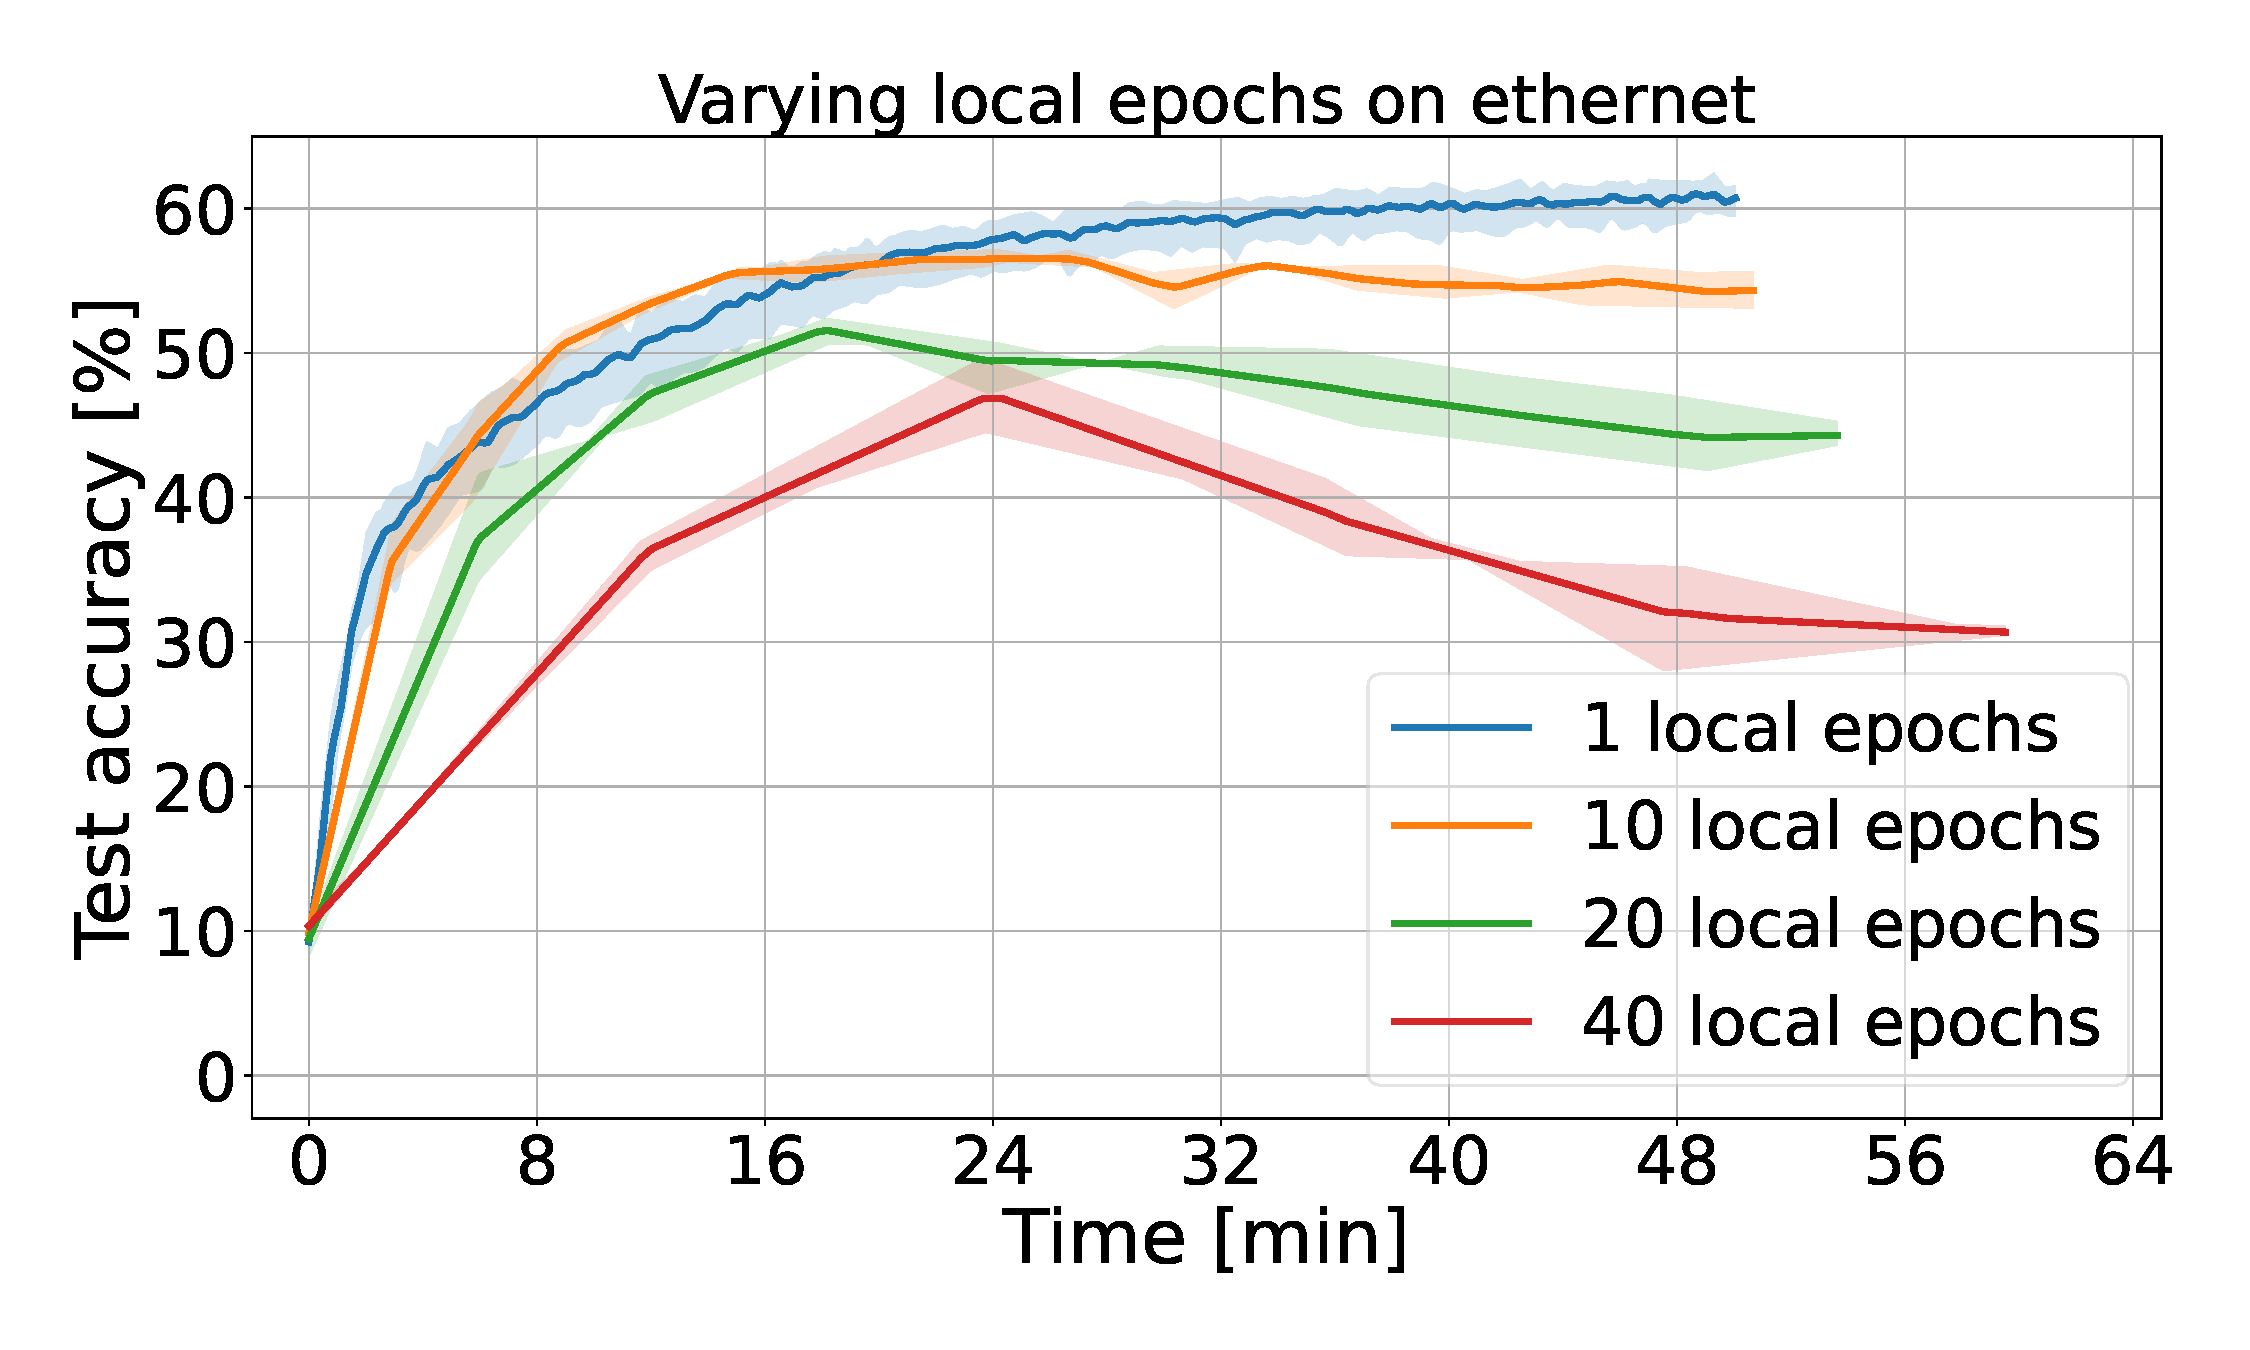
\includegraphics[width=.49\linewidth]{imgs/time_avg_local_epochs_ethernet.pdf}
        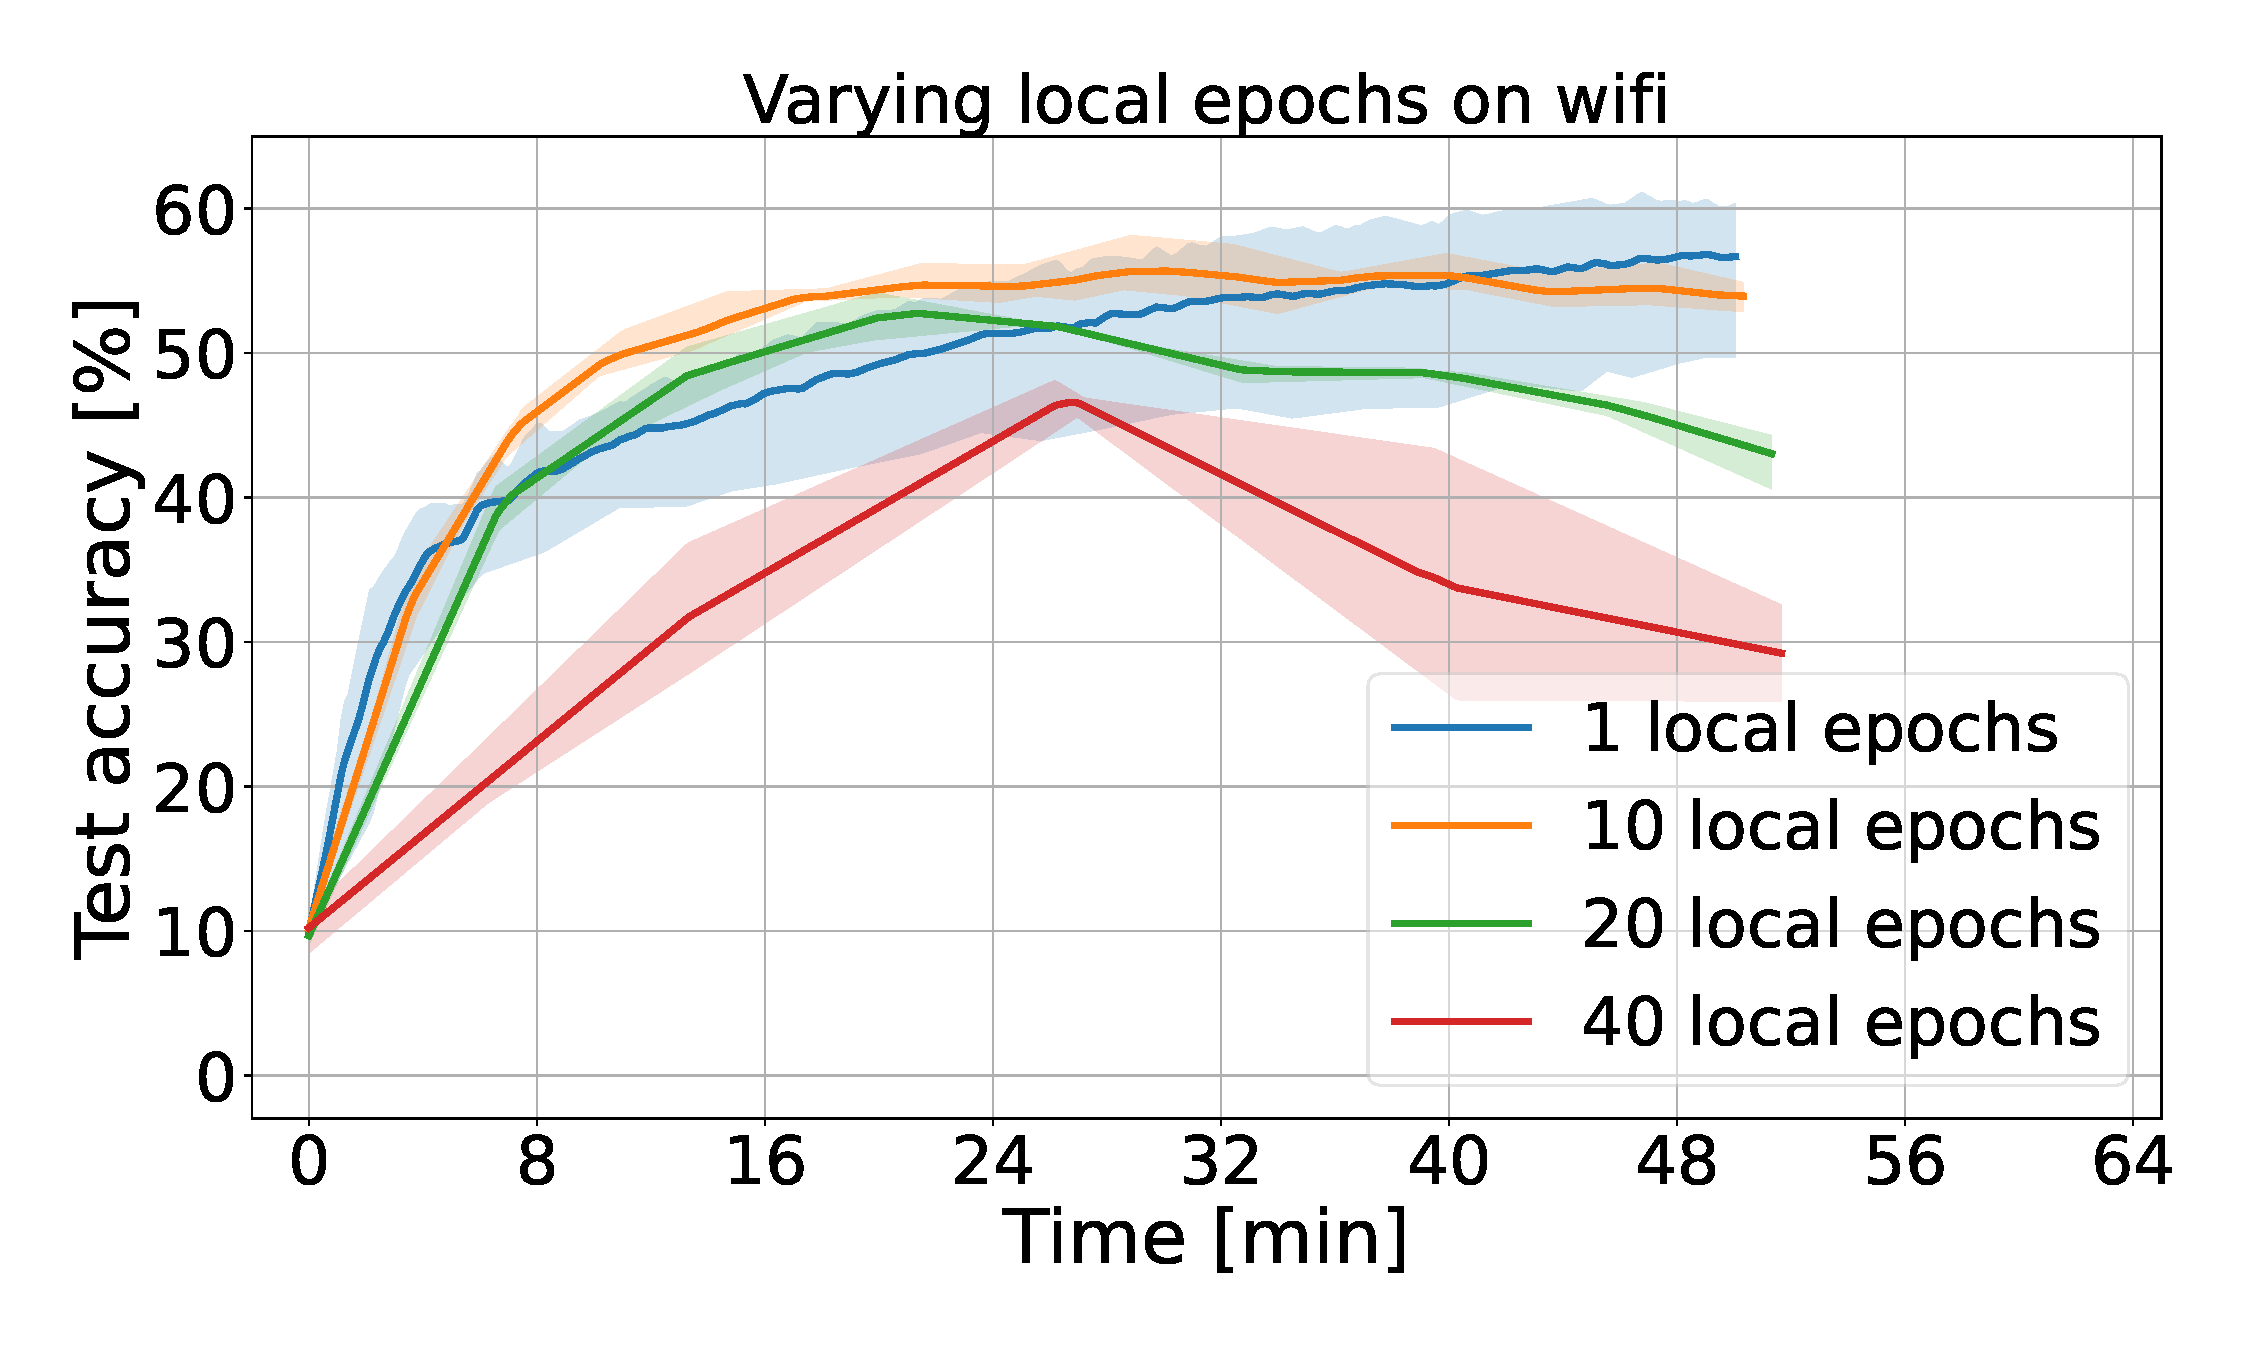
\includegraphics[width=.49\linewidth]{imgs/time_avg_local_epochs_wifi.pdf}
    \end{figure}\noindent
\end{frame}

\begin{frame}
\frametitle{A Practical Case Study, But...}
    \small
    \begin{itemize}
        \item This is just one setup
        \item Simple model with simple dataset
        \item Little focus on regularization
    \end{itemize}
    Our experiment highlights tradeoffs and considerations for practical applications, but severity and good design choices will vary.
    \begin{figure}[H]
        \centering
        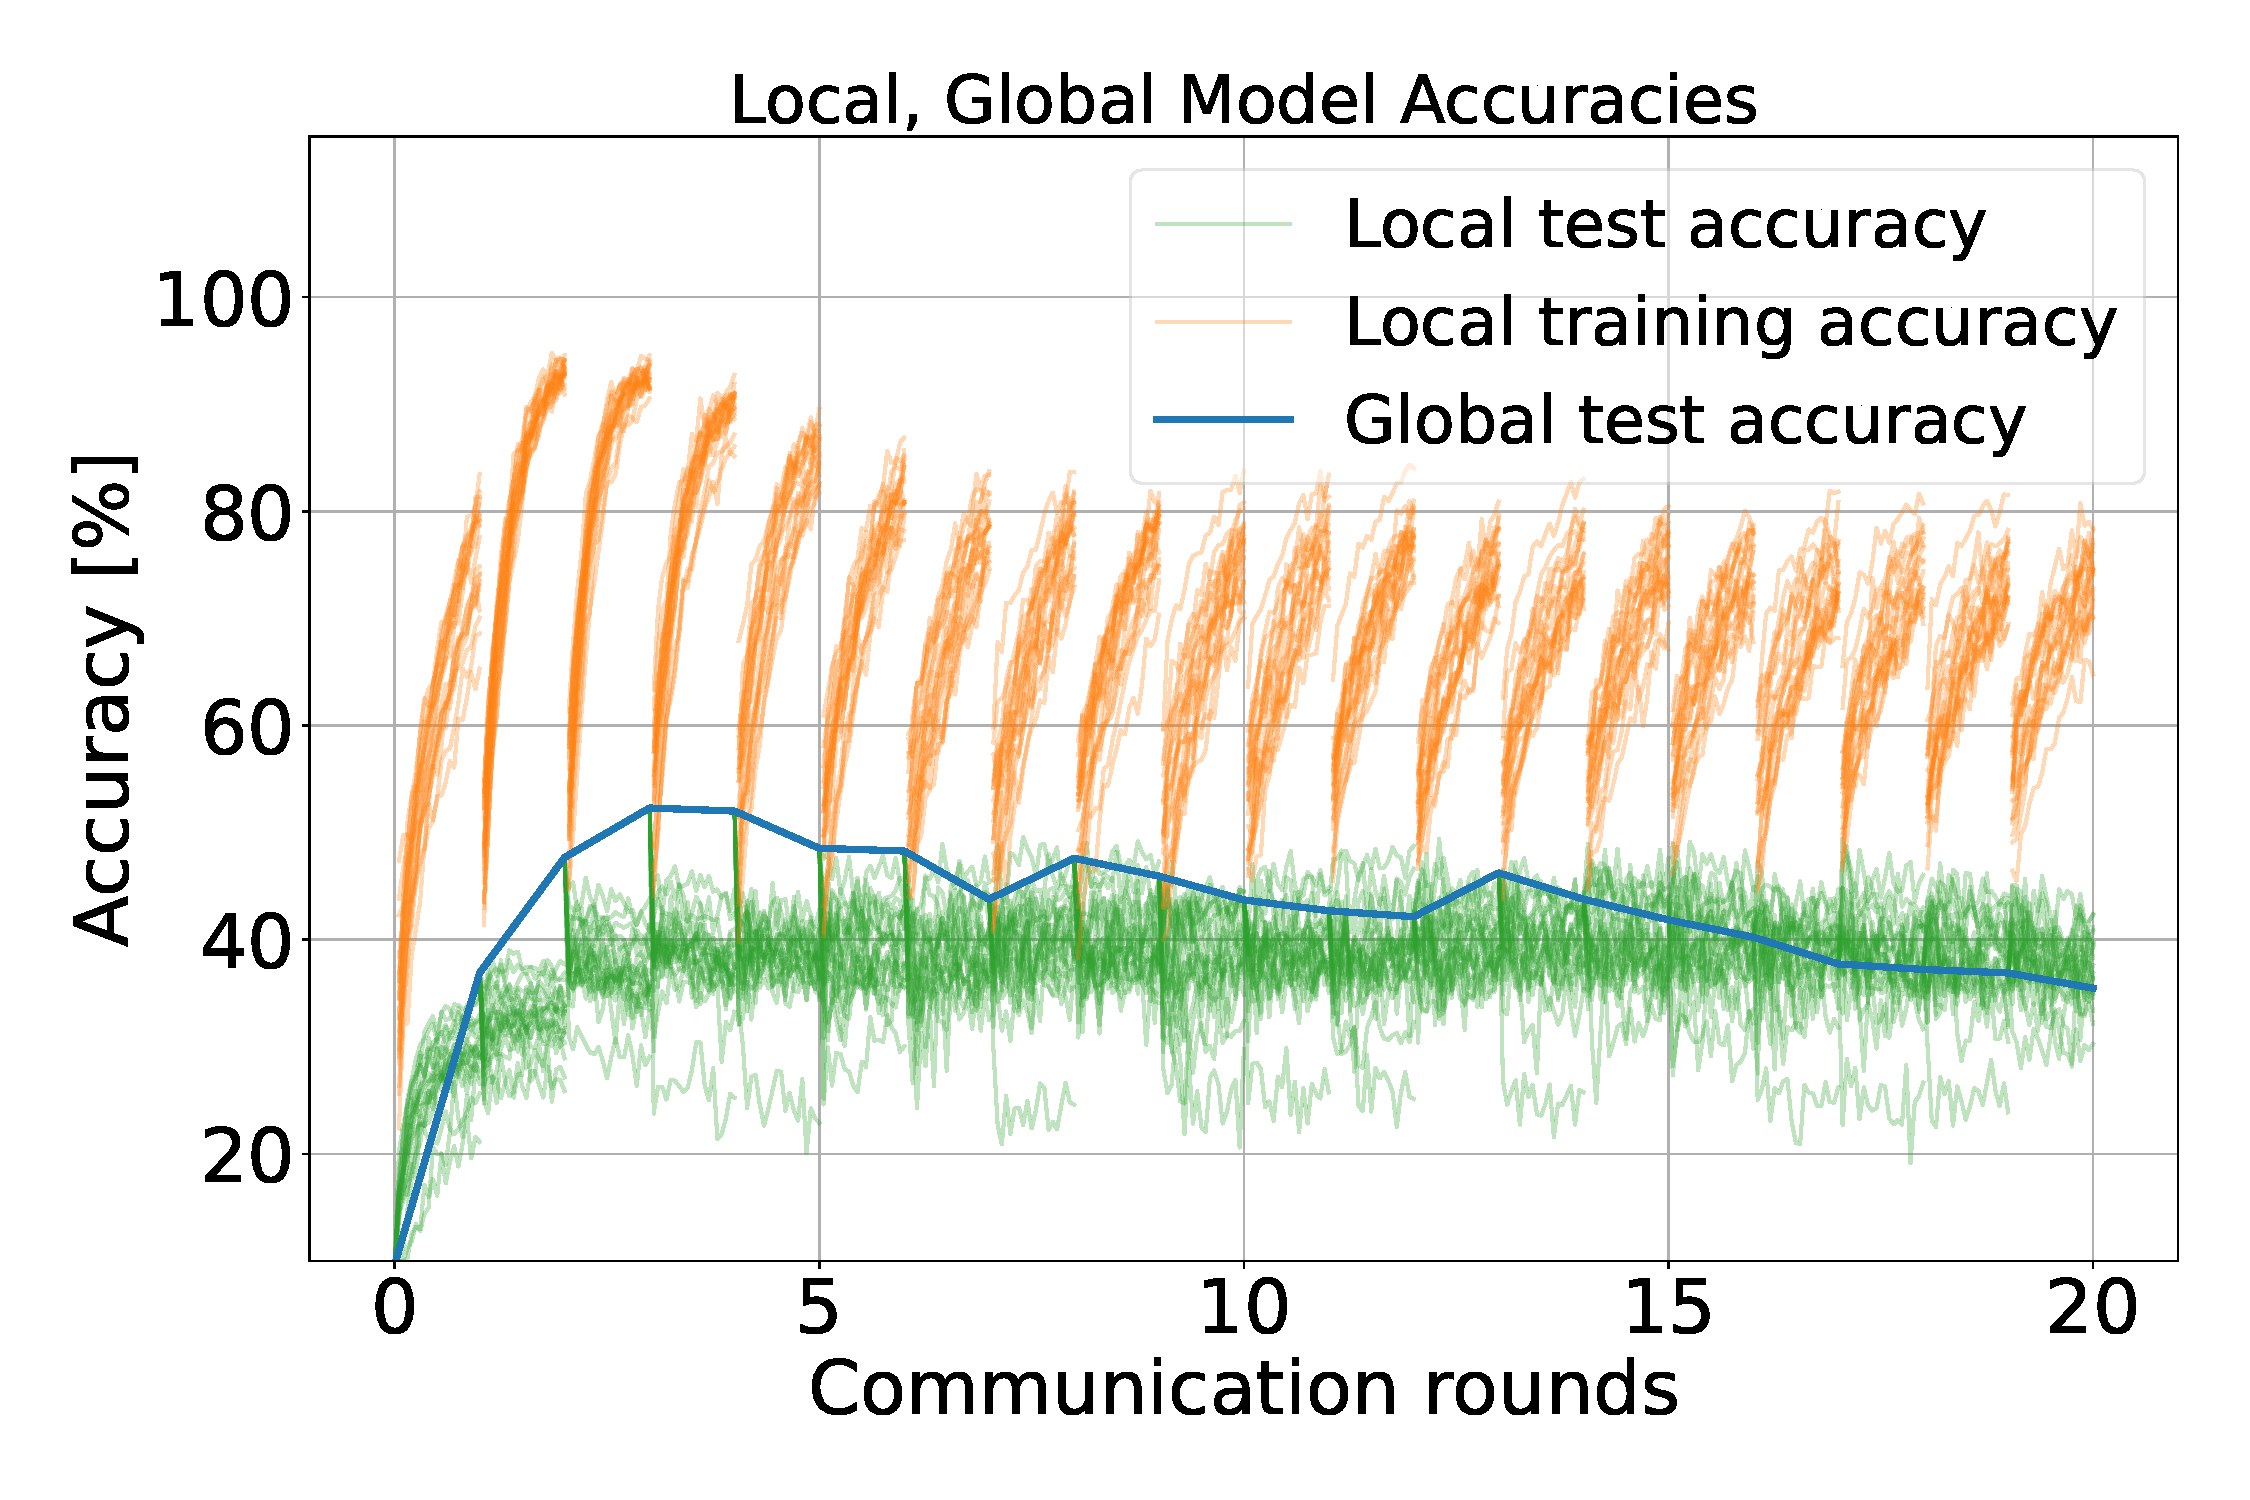
\includegraphics[width=.49\linewidth]{imgs/accuracy.pdf}
        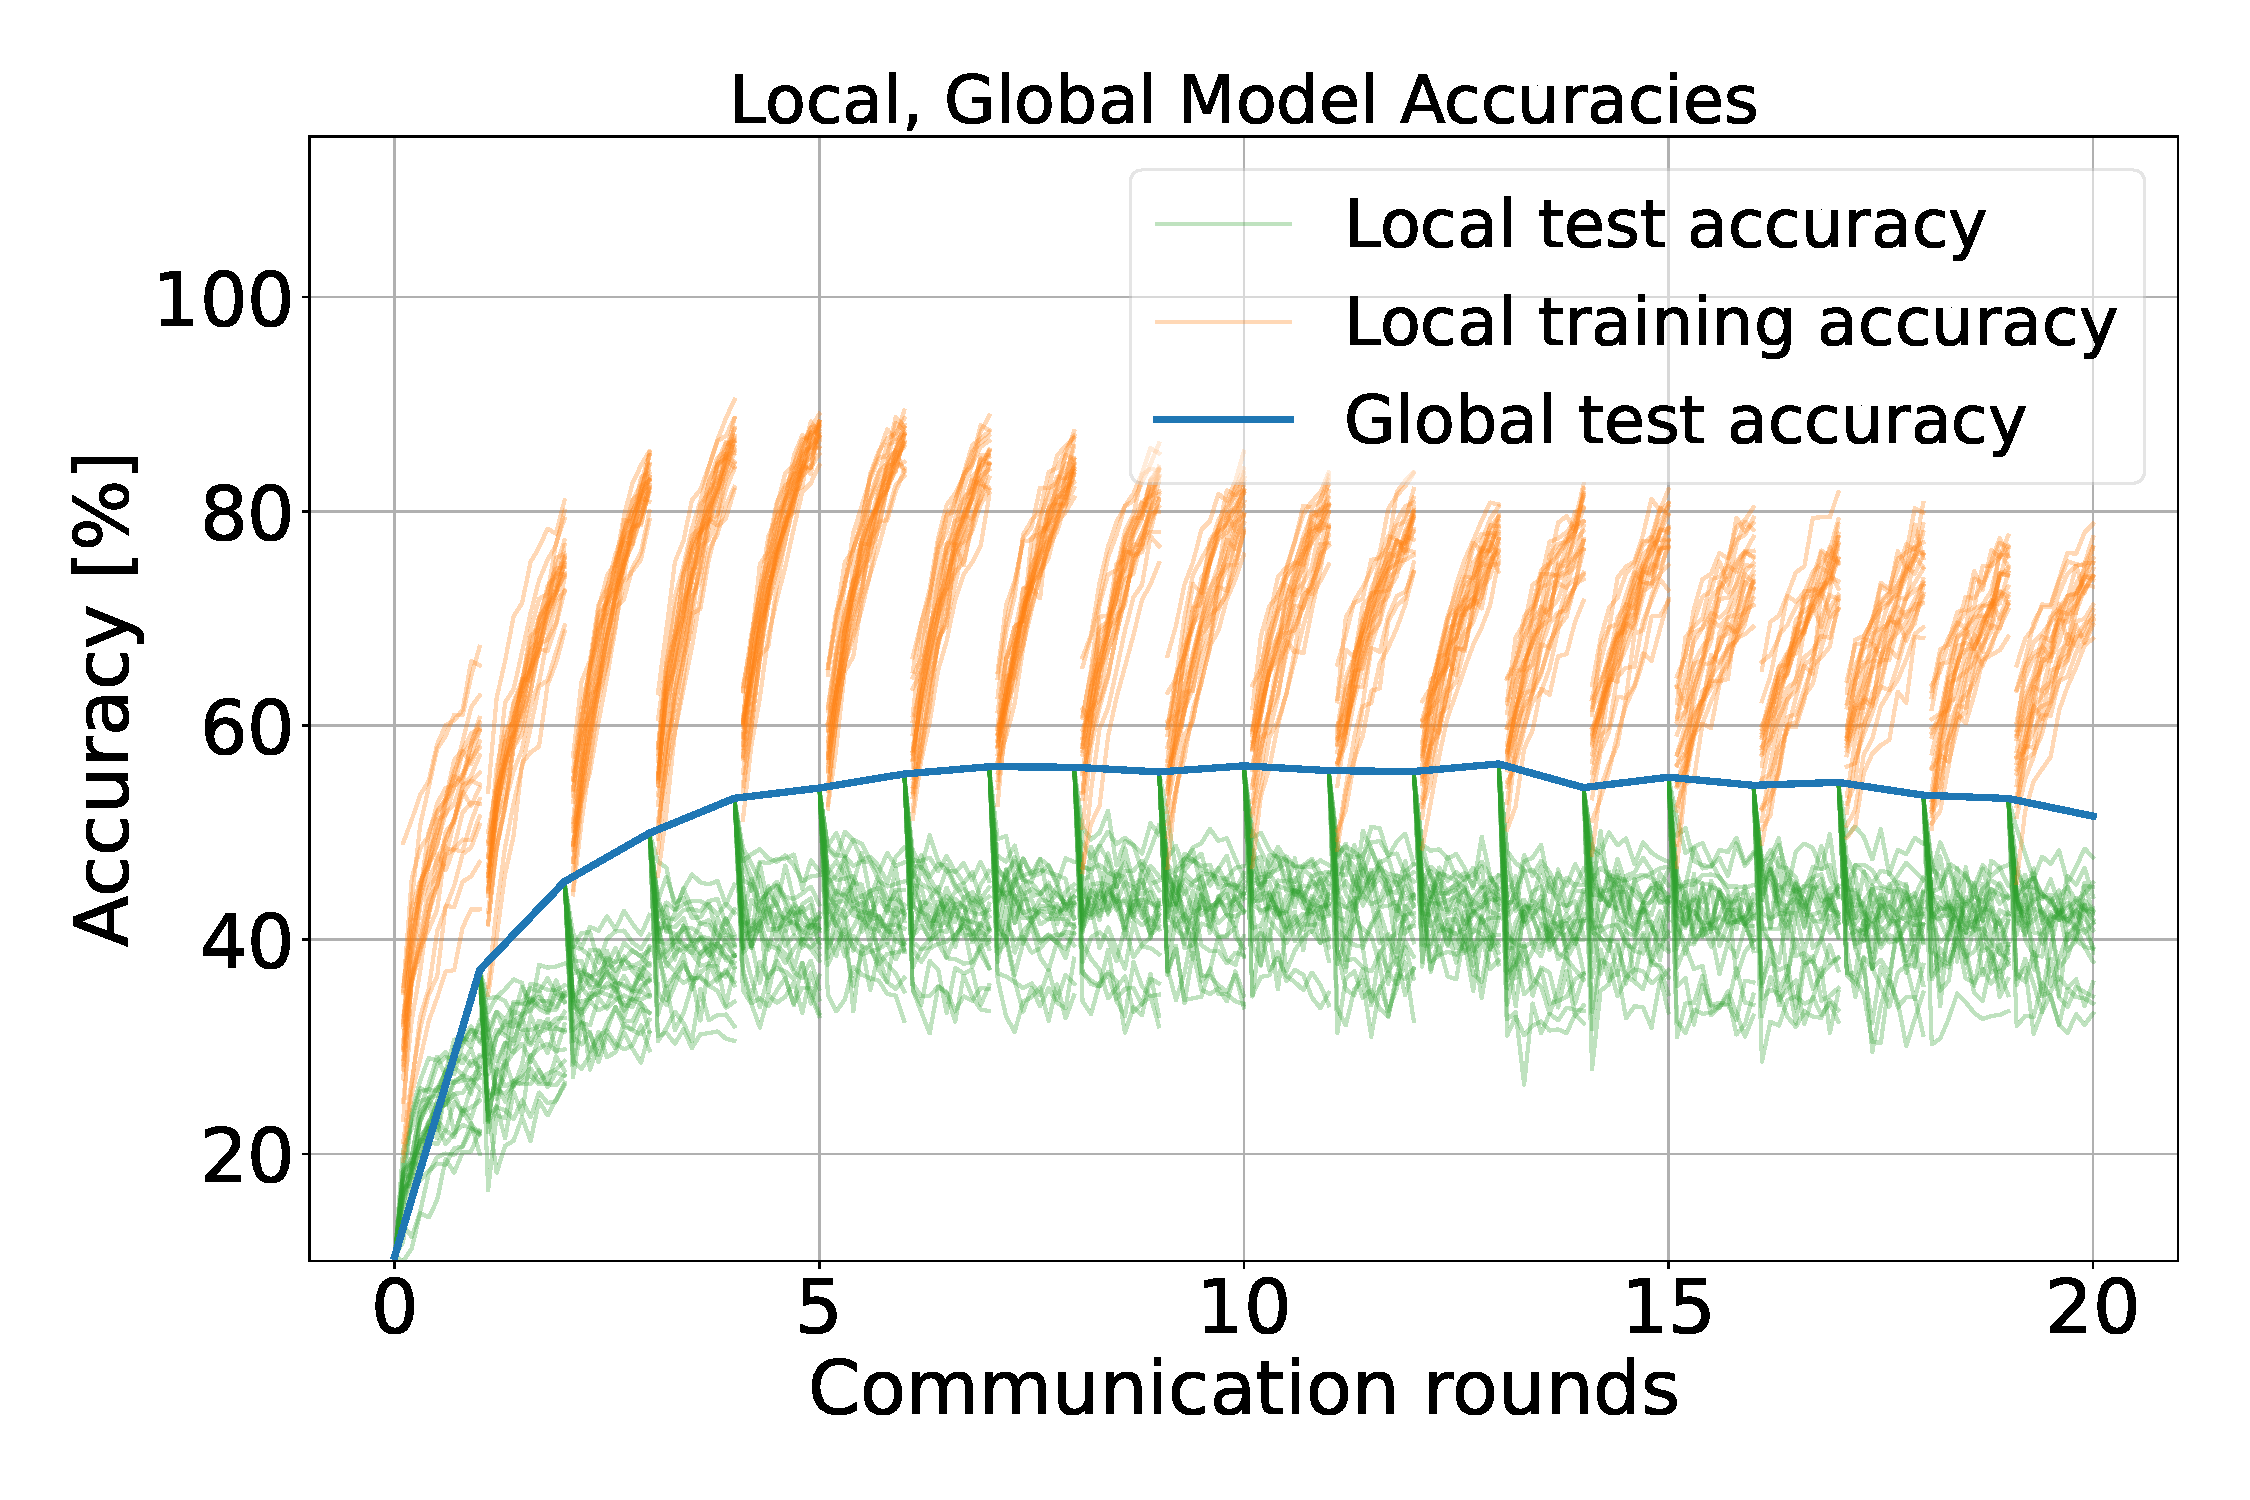
\includegraphics[width=.49\linewidth]{imgs/accuracyE10.pdf}
    \end{figure}\noindent
\end{frame}

\section{Robust Aggregation Using FedDF}
\begin{frame}
    \frametitle{Federated Robustness}
    \begin{itemize}
        \item World of theory: IID, no label noise
        \item Weight averaging $\Rightarrow$ all client datasets are equal
        \item "The characterization of cross-client differences in real-world partitioned datasets is an important open question" [Ch. 3.1, 1]
    \end{itemize}

    \begin{example}[GBoard Users]
        \begin{itemize}
            \item User 1: Long, professional emails
            \item User 2: Angry YouTube comments
            \item User 3: In Dutch, accidentally combined with English data
        \end{itemize}
    \end{example}
\end{frame}

\begin{frame}
    \frametitle{The FedDF Algorithm}
    \begin{algorithm}[H]
    \caption{FedDF}
    \label{alg:dir}
    \scriptsize
    \begin{algorithmic}
    \For{$l$ from 1 to $L$}
    \For{$s$ from 1 to $S$ in parallel}
        \State{
            $\mathcal M^{(l)}_{k_s} \gets \mathcal M^{(l)}_G$, then train $\mathcal M^{(l)}_{k_s}$ locally for $E$ epochs on partition $k_s$
        }
    \EndFor
    \State{
        $e_\text{old} \gets \infty, e_\text{new} \gets \infty, i \gets 0$
    }
    \State{
        $\mathcal M^{(l+1)}_G \gets \frac 1 S \sum_{s=1}^S \mathcal M^{(l)}_{k_s}$
    }
    \While{$e_\text{new} \leq e_\text{old}$ for up to $10^4$ iterations}
    \State{
        Sample batch $\bm{\mathcal B}$ from distillation dataset
    }
    \State{
        $\mathbf T \gets \sigma(\frac 1 S \sum_{s=1}^S \mathcal M^{(l)}_{k_s}(\bm{\mathcal B}))$\Comment{Sigmoid of avg. client logits}
    }
    \State{
        $\mathcal M^{(l+1)}_G \gets \mathcal M^{(l+1)}_G - 
        \frac{\partial 
            \operatorname{KL}{\left(
                \mathbf T, \sigma(\mathcal M^{(l+1)}_G(\bm{\mathcal B}))
    \right)}}
            {\partial M^{(l+1)}_G }$
        } \Comment{Grad. of KL (Actually ADAM)}
        \If{iteration is multiple of $10^3$}
        \State{
            $e_\text{old} \gets e_\text{new}$, $e_\text{new} \gets$ Average KL Div. over test set
        }
        \EndIf
    \EndWhile
    \EndFor
    \end{algorithmic}
    \end{algorithm}
\end{frame}

\begin{frame}
    \frametitle{Data Imbalance}
    \begin{figure}[H]
        \centering
	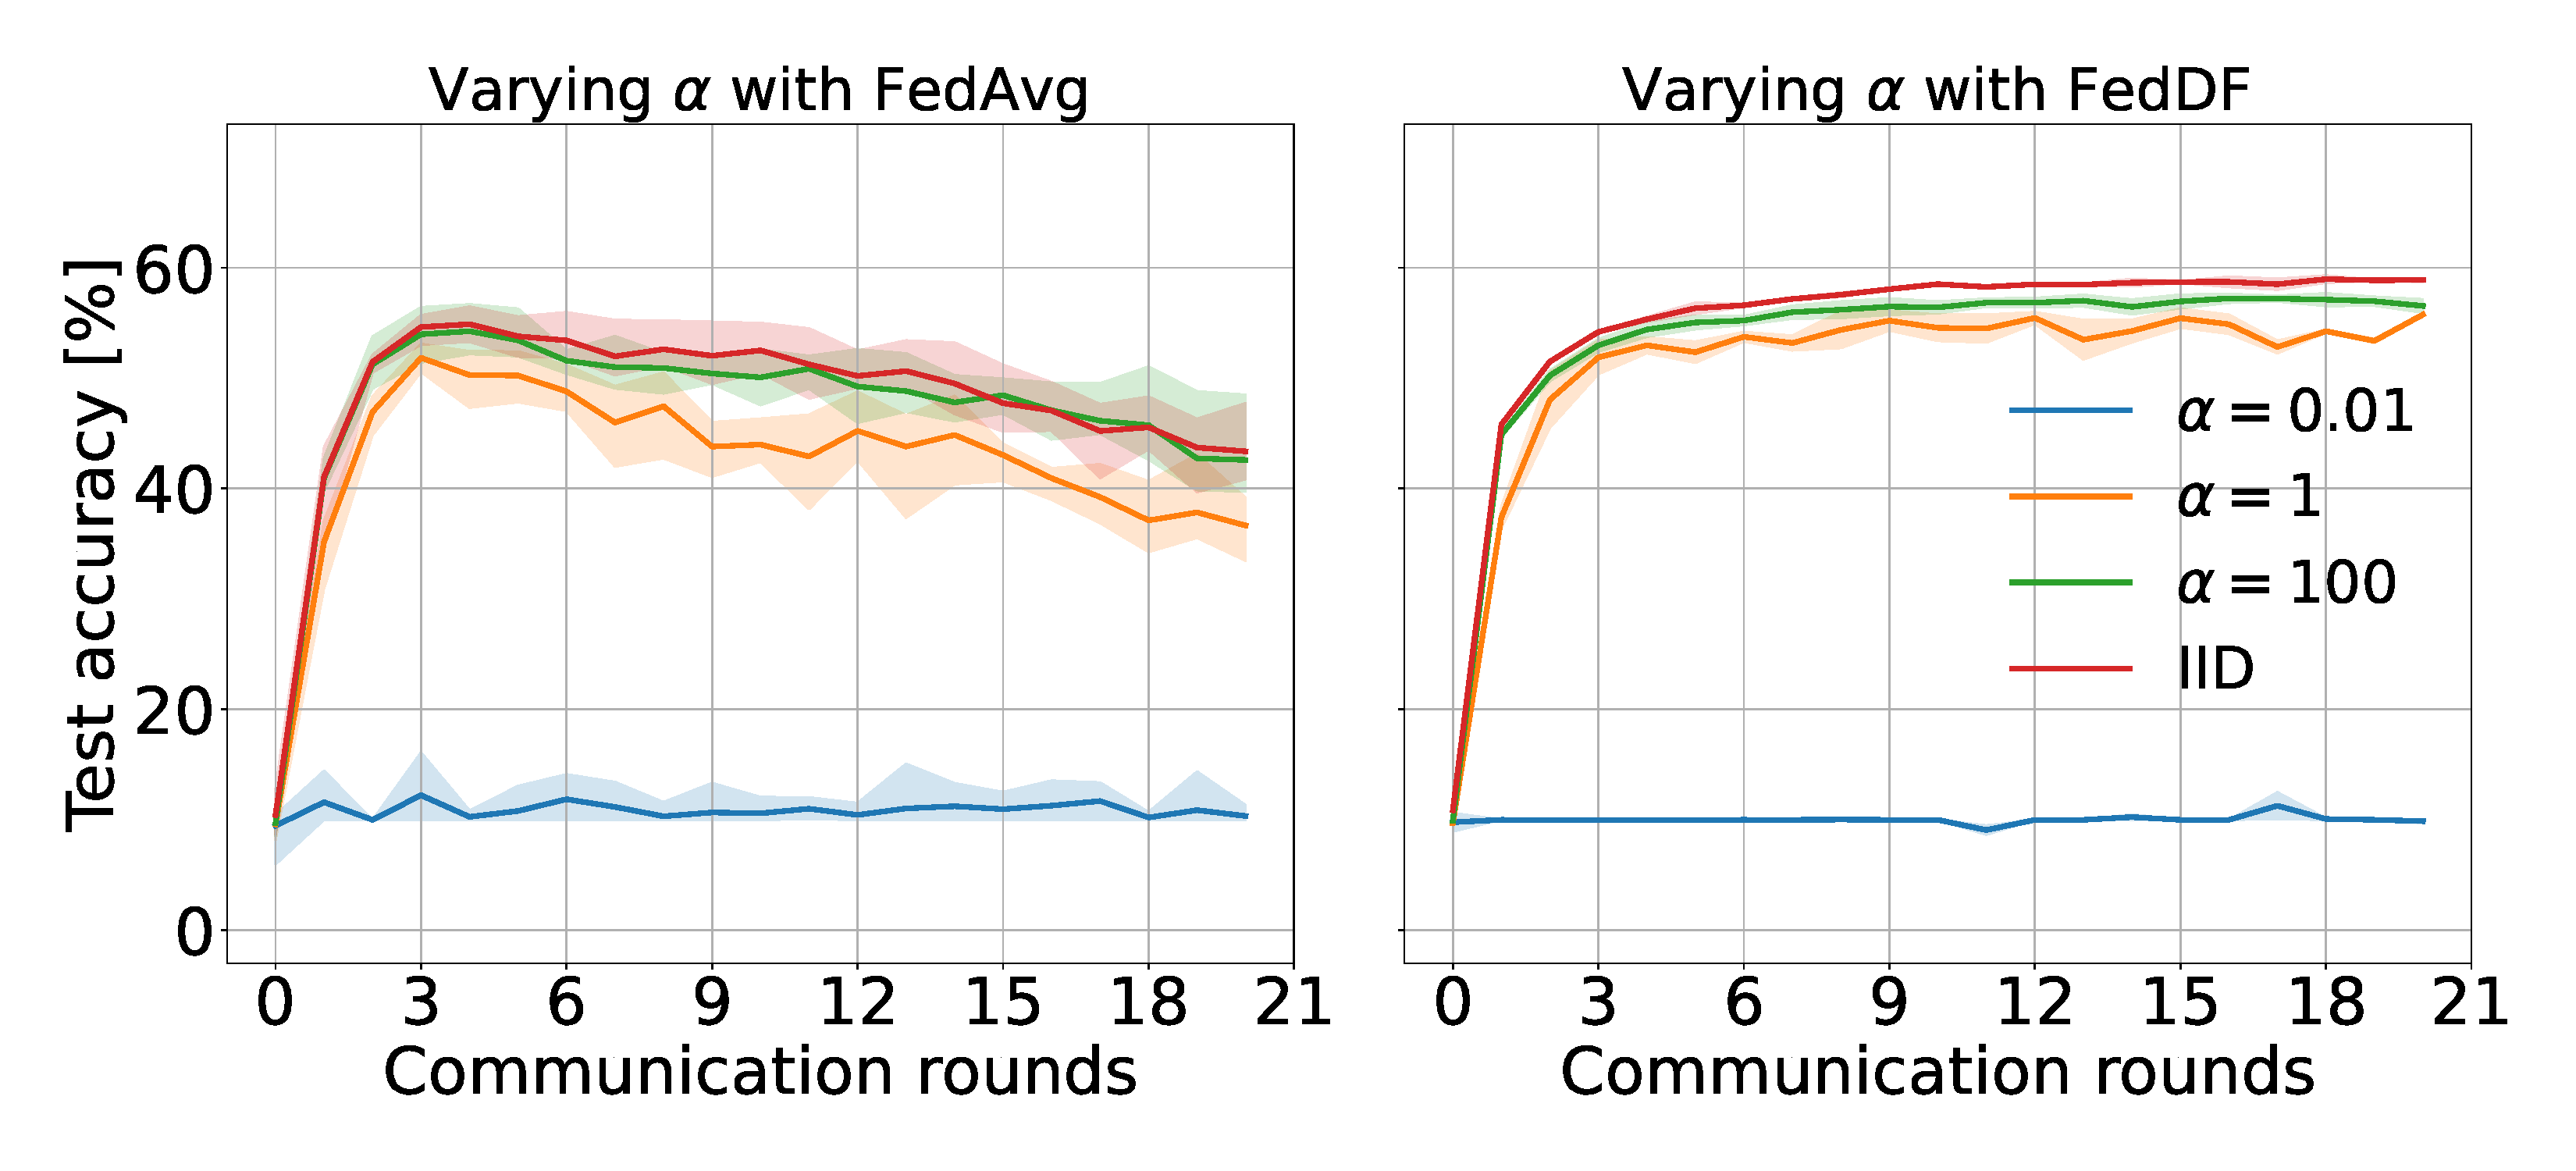
\includegraphics[width=.7\linewidth]{imgs/feddf-alpha.pdf}
    \end{figure}\noindent

\begin{table}[htb!]
    \centering
    \footnotesize
    \begin{tabular}{llll}
       \hline
        \multicolumn{4}{c}{Class balance ($\alpha$)}\\
        0.01 & 1.0 & 100.0 & iid. \\
       \hline
        $10.3 \pm 0.6$ & $36.7 \pm 2.4$ & $42.6 \pm 3.4$ & \textbf{ 43.4 $\pm$ 2.5  }\\
        \multicolumn{4}{c}{FedDF: Class balance ($\alpha$)}\\
        0.01 & 1.0 & 100.0 & iid. \\
       \hline
        $9.9 \pm 0.2$ & $55.8 \pm 0.1$ & $56.5 \pm 0.9$ & \textbf{ 58.3 $\pm$ 1.0 } \\
\end{tabular}
    \caption{
	Test accuracy [\%] after 20 rounds.
    }
\end{table}
\end{frame}
\begin{frame}
    \frametitle{Noisy Clients}
    \begin{figure}[H]
        \centering
	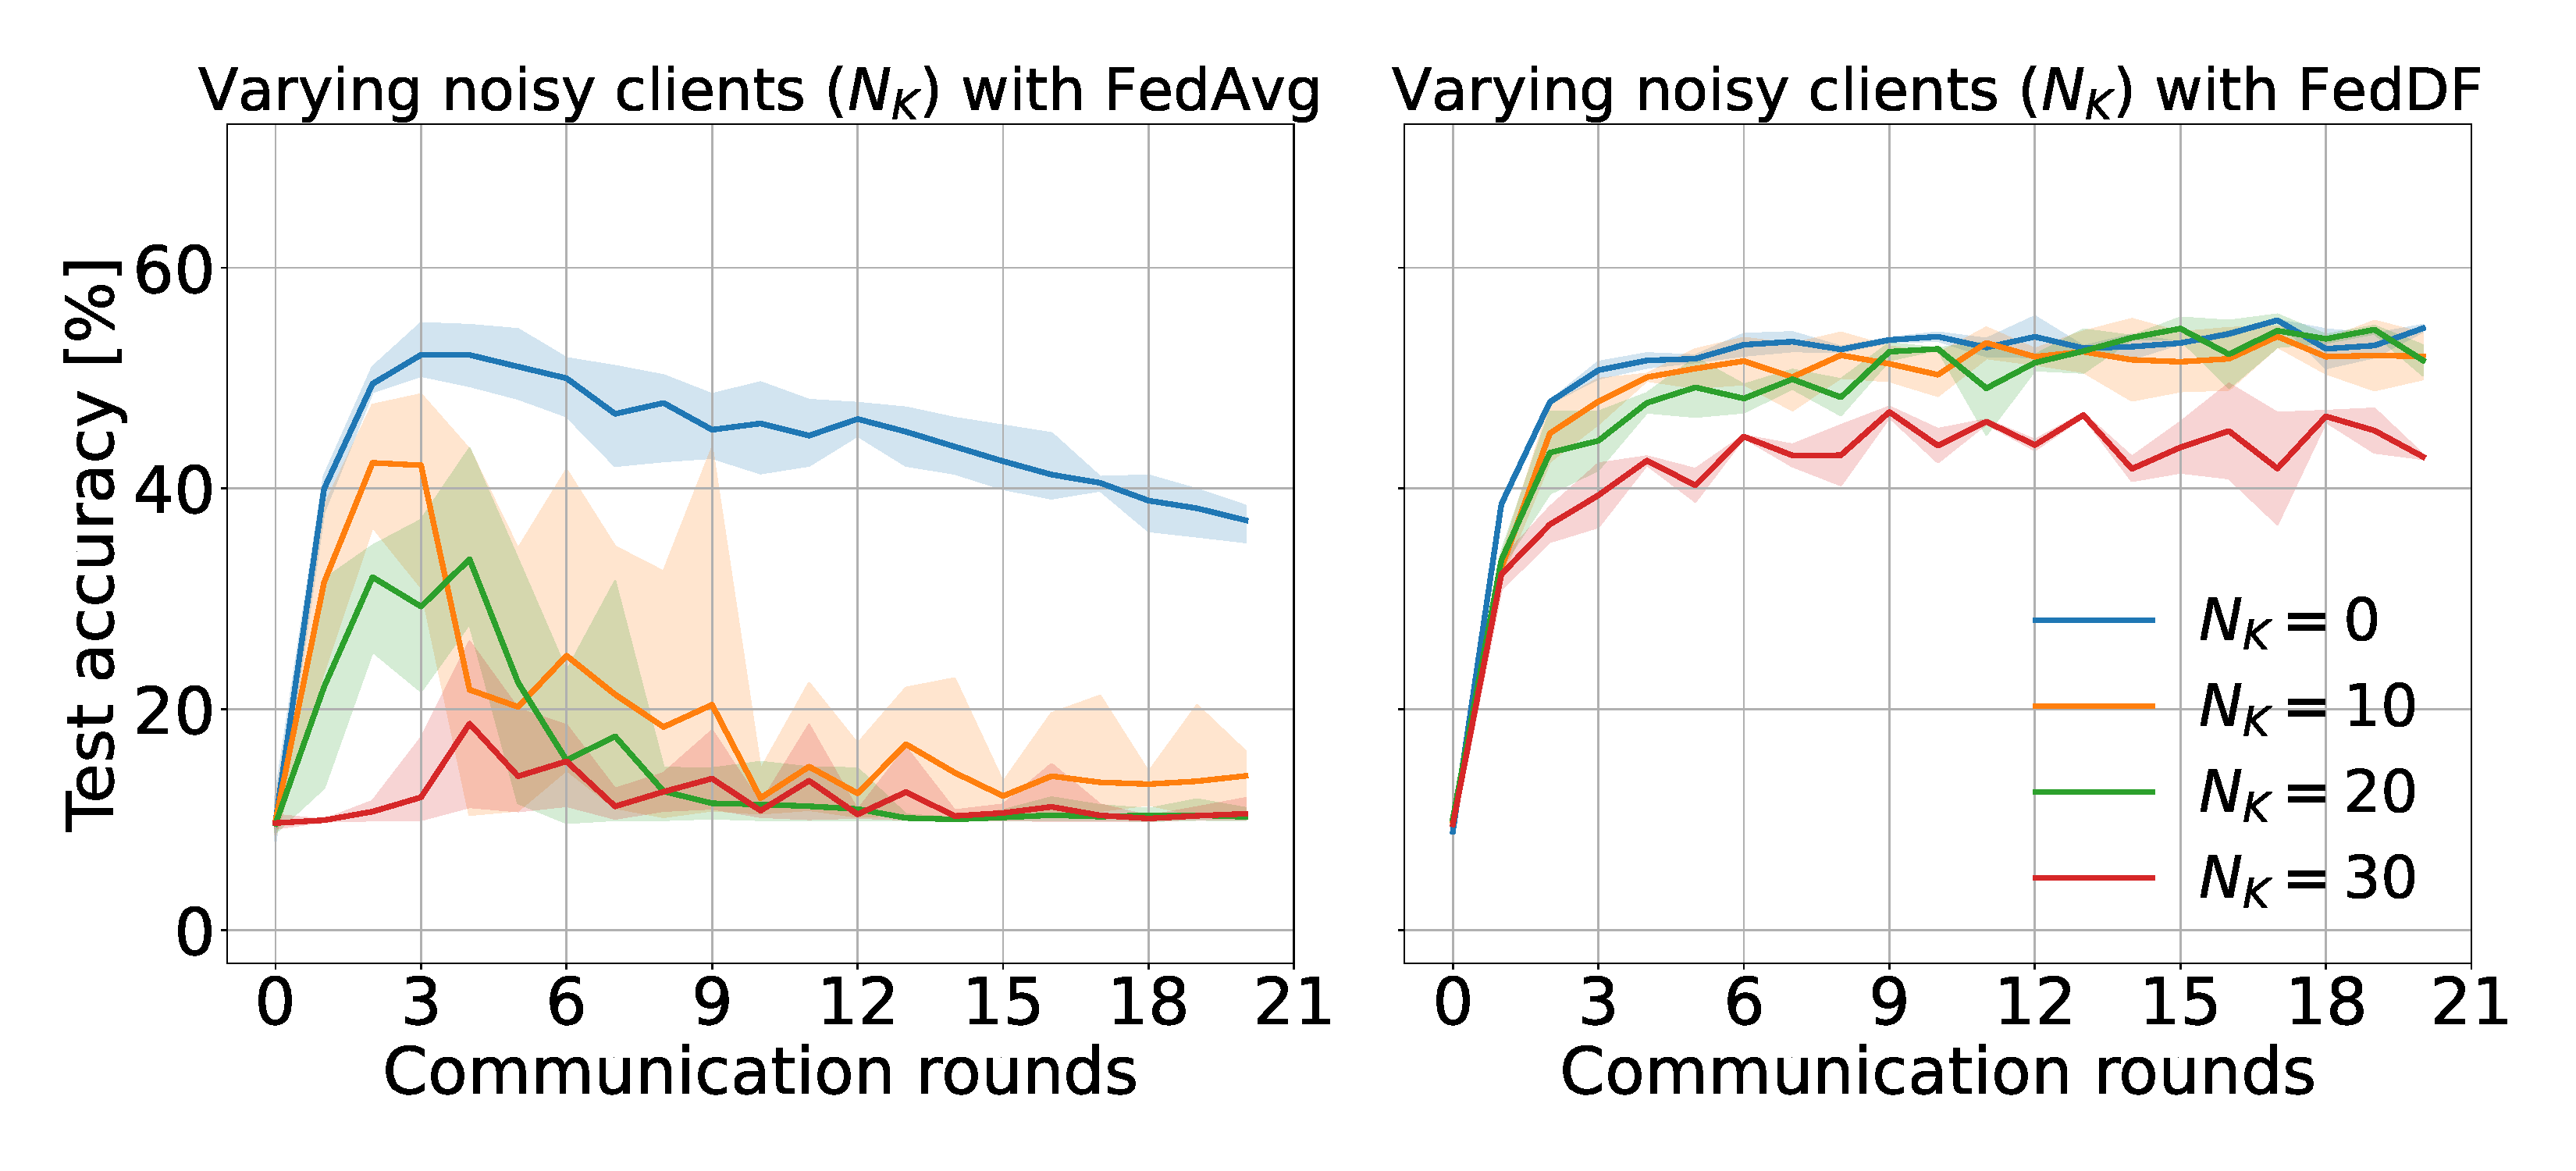
\includegraphics[width=.7\linewidth]{imgs/noisy_clients.pdf}
    \end{figure}\noindent
\begin{table}[htb!]
    \centering
    \footnotesize
    \begin{tabular}{llll}
       \hline
        \multicolumn{4}{c}{Noisy clients ($N_K$)}\\
        0 & 10 & 20 & 30 \\
       \hline
        \textbf{ 37.1 $\pm$ 1.3 } & $14.0 \pm 2.1$ & $10.3 \pm 0.4$ & $10.6 \pm 0.8$ \\
        \multicolumn{4}{c}{FedDF: Noisy clients ($N_K$)}\\
        0 & 10 & 20 & 30 \\
       \hline
        \textbf{ 54.5 $\pm $ 0.4 } & $52.0 \pm 2.9$ & $51.6 \pm 1.9$ & $42.9 \pm 0.3$ \\
\end{tabular}
    \caption{
    Final test accuracies [\%], 5 repetitions, 95\%\ CI.
    }
\end{table}
\end{frame}




\end{document}
